\documentclass[a4paper,12pt]{report}
\usepackage[T1]{fontenc}
\usepackage[utf8]{inputenc}
\usepackage{lmodern}
\usepackage{amsmath}
\usepackage{amsfonts}
\usepackage{amssymb}
\usepackage{amsthm}
\usepackage{graphicx}
\usepackage{color}
\usepackage{xcolor}
\usepackage{url}
\usepackage{textcomp}
\usepackage{parskip}
\usepackage{setspace}
\usepackage{hyperref}

% source:
% https://blog.visual-paradigm.com/fr/the-four-types-of-relationship-in-use-case-diagram/
% https://firebase.google.com/
% https://coolors.co/
% https://app.diagrams.net/
% https://vuefire.vuejs.org/
% https://www.overleaf.com/
% https://www.latex-fr.net/3_composition/texte/paragraphes/modifier_l_interligne

\title{Implémentation d'une application de gestion de tache}
%\author{NKWE AHOUME BORIS}
\author{
  M. FOKOU KEMEGNE - Encadreur Académique\\
  %\texttt{first1.last1@xxxxx.com}
  \and
  M. HANNIEL TSASSE - Encadreur Professionel(FAROTY S.A.S)\\
  \and
  NKWE AHOUME BORIS - Etudiant en Genie Logiciel\\
  \texttt{nkabo074@gmail.com}
}


\date{\today}

\setstretch{1.5} % interline

\begin{document}

% Where the title will be.
\maketitle

% definition
\def\chaptername{Chapitre}% definie le titre du chapitre en FR
\def\listfigurename{Liste des figures}
\def\contentsname{Somaire}


\renewcommand{\abstractname}{Dedicace}
\begin{abstract}
À mes parents, qui m'ont toujours soutenu et encouragé à poursuivre mes rêves. Merci de croire en moi.
\end{abstract}

\renewcommand{\abstractname}{Remerciment}
\begin{abstract}
Je souhaite exprimer ma profonde gratitude à toutes les personnes qui ont contribué à la réalisation de ce mémoire. Tout d'abord, je remercie Dieu Tout-Puissant pour m'avoir accordé la force, la sagesse et la persévérance nécessaires pour mener à bien ce projet.
Je tiens à remercier chaleureusement:

\begin{itemize}
  \item le Directeur de l'Institue Universitaire de technologie de Douala pour le soutien institutionnel et les opportunités académiques offertes tout au long de mon parcours. Mes remerciements vont également au 
  \item Responsable Académique M. MBAI, dont les conseils avisés et le dévouement ont été précieux.
  \item Mes parents, pour leur amour inconditionnel, leur soutien moral et financier, et leurs encouragements constants qui ont été une source inestimable de motivation.
  \item Mes frères et sœurs, je suis reconnaissant pour leur soutien affectueux et leur compréhension durant les moments difficiles.
  \item Mon Encadreur Professionnel M. HANNIEL TSASSE, dont l'expertise et les conseils pratiques m'ont guidé tout au long de cette recherche. 
  \item Mon Encadreur Académique M. FOKOU KEMEGNE mérite aussi une reconnaissance particulière pour son accompagnement pédagogique, sa patience et ses précieux conseils.
\end{itemize}

Un grand merci à 
Je remercie également

\begin{itemize}
  \item[•] mes professeurs, qui ont partagé leur savoir et leur passion, contribuant ainsi de manière significative à ma formation.
  \item[•] merci sincère à mes camarades, pour leur soutien, leur camaraderie et les moments partagés qui ont rendu cette expérience mémorable et enrichissante.
\end{itemize}

À vous tous, merci infiniment.
\end{abstract}

% Where the table of contents will be.
\tableofcontents

\renewcommand{\abstractname}{Résumé}
\begin{abstract}
Le présent rapport détaille la conception et le développement d'une application de gestion de tâches, nommée GETDO pour le compte de la société FAROTY SAS. L'objectif principal de cette application est d'aider les utilisateurs à organiser efficacement leurs tâches quotidiennes, à suivre leur progression et à améliorer leur productivité.
L'application propose plusieurs fonctionnalités clés, notamment l'assignation de tâches avec des dates d'échéance, un tri en fonction des priorités, des rappels,un calendrier, un suivi de l'accomplissement des tâches, un tableau de vision pour visualiser les objectifs à long terme, ainsi qu'un tableau de bord offrant une vue d'ensemble de la progression des tâches à l'aide de graphiques.
Le développement de l'application s'est appuyé sur des technologies modernes telles que Vue JS pour le front-end et FireBase pour le back-end, offrant ainsi une expérience utilisateur fluide et intuitive. De plus,l'application fonctionnalités avancées telles que une optimisation de la planification et une analyse de productivité.
Ce rapport décrit en détail le processus de conception, de développement et de test de l'application, ainsi que les défis rencontrés et les solutions apportées. En outre, il met en évidence les perspectives d'amélioration et les pistes pour de futures recherches et développements dans le domaine de la gestion de tâches et des possibilité de l'intégration de l'Intelligence Artificielle.
En conclusion, l'application GETDO représente une contribution significative dans le domaine de la gestion de tâches, offrant aux utilisateurs une solution moderne et efficace pour gérer leur travail et améliorer leur productivité au quotidien.
\end{abstract}

% liste des figures
\listoffigures

% Introduction générale
\chapter*{Introduction Générale}
Dans un monde où le temps et les ressources sont des éléments précieux, la gestion efficace des tâches et des projets revêt une importance capitale pour les individus et les organisations. Dans ce contexte, les applications de gestion de tâches jouent un rôle essentiel en offrant des outils et des fonctionnalités permettant de planifier, suivre et organiser les activités quotidiennes et les projets à long terme de manière efficace et méthodique.
Le présent rapport détaille le processus de conception et de développement d'une application de gestion de tâches moderne, intitulée GETDO. Notre objectif principal est de fournir aux utilisateurs une solution robuste et intuitive pour gérer leurs tâches personnelles et professionnelles, en mettant l'accent sur l'optimisation de la productivité, la facilitation de la collaboration et l'amélioration de l'efficacité opérationnelle.
Ce rapport présentera en détail les différentes phases du projet, depuis la phase de conception initiale jusqu'au déploiement final de l'application. Nous aborderons les aspects techniques, fonctionnels et conceptuels du développement, en mettant en lumière les défis rencontrés, les solutions apportées et les choix technologiques effectués tout au long du processus.
De plus, nous explorerons les opportunités offertes par l'intégration de l'intelligence artificielle dans notre application, en examinant comment les fonctionnalités avancées telles que les recommandations intelligentes, l'analyse de données et l'automatisation peuvent contribuer à améliorer l'expérience utilisateur et à optimiser la gestion des tâches.
Enfin, nous discuterons des perspectives d'avenir pour notre application, en identifiant les pistes pour de futures améliorations, les évolutions technologiques envisagées et les possibilités d'extension et d'adaptation pour répondre aux besoins changeants des utilisateurs et du marché.
À travers ce rapport, nous espérons fournir un aperçu complet de notre travail et de notre vision pour l'application GETDO, ainsi que de son potentiel à contribuer à l'efficacité et à la réussite des individus et des organisations dans leur gestion quotidienne des tâches et des projets.

% presentation de l'entreprise
\chapter{Présentation de l'entreprise FAROTY SAS} 
FAROTY SAS est une société camerounaise innovante qui offre des solutions financières numériques à une clientèle grandissante. Localiser a près de l’hôtel Kremlin a Bonamousadi, FAROTY a pour mission de faciliter l'accès aux services financiers de base pour tous les Camerounais, en particulier ceux des zones rurales et non bancarisées.
FAROTY propose une suite complète de solutions financières numériques, notamment :
\begin{itemize}
  \item[•] Paiements et transferts d'argent : Envoyez et recevez de l'argent facilement et en toute sécurité via des plateformes de paiement mobile et électronique (Orange Money, MTN Mobile Money, PayPal). 
  \item[•] Gestion financière personnelle : Gérez vos finances personnelles en toute simplicité avec nos outils de budgétisation, de suivi des dépenses et d'épargne. 
  \item[•] Collecte de fonds (Crowdfunding) : Levez des fonds pour vos projets et causes grâce à notre plateforme de crowdfunding sécurisée. 
  \item[•] Tontines digitales : Participez à des tontines virtuelles et gérez vos cotisations en ligne. 
  \item[•] Billetterie électronique : Achetez et vendez des billets d'événements en ligne avec notre service ePass. 
  \item[•] Pages commerciales : Créez votre propre boutique en ligne et vendez vos produits et services facilement. 
  Leurs technologie
\end{itemize} 
FAROTY a un impact positif sur les Camerounais en leur offrant un accès plus facile aux services financiers il est donc de notre devoir de facilité leurs travails via l'application présenter dans ce rapport

% Presentationde de l'equiment utiliser, et des methodes
\chapter{Méthode et equipements utilisé}
\section{équipement et logiciel utiliser}

Pour mener à bien ce projet, plusieurs outils technologiques ont été utilisés. Voici les principaux :
\begin{itemize}
  \item\textbf{Logiciel de design:} Lunacy
  \item\textbf{Logiciel de modelisation:} draw.io
  \item\textbf{IDE}: Visual Studio Code est l'editeur de choix pour notre project.
  \item\textbf{Syteme de controle de version}: Git et Github.
  \item\textbf{Langages de Programmation et technologie}: JavaScript pour front-end(Vue.JS) et FireBase en back-end.
\end{itemize}

\section{Méthode utilisé}
Comme méthode utiliser, nous avont opter pour la méthode de dévélopement agile SCRUM et la modelisation UML. Chaque tâches sont séparé en sprint, et à la fin de chacun d'entre eux, un livrable est fournie. La liste des livrables et de l'application elle meme attendues pour ce project sont:
\begin{itemize}
  \item L'Application de gestion de tâche GETDO.
  \item Creation de tâche.
  \item Vision Board.
  \item Tableaux de bord et visualisations de données.
  \item Prise en charge d'un styles de gestion des tâches.
\end{itemize}

\subsection{Mise en place des outils de gestion de project}
Pour assuré la gestion bonne gestion du project, nous allons utiliser le logiciel de gestion JIRA

% Jira screenshot 
\begin{figure}[h!]
    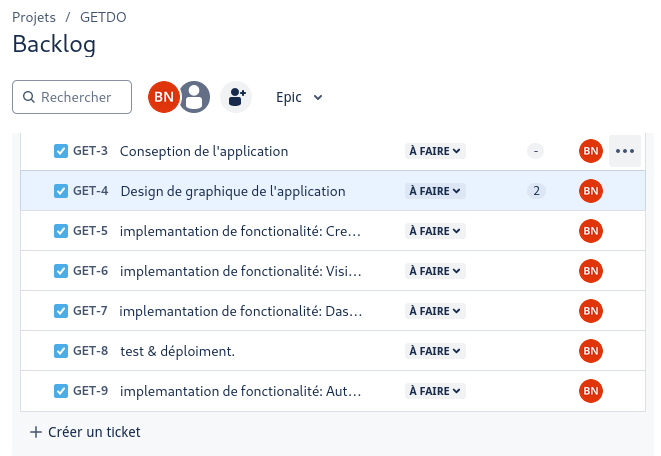
\includegraphics[width=1\textwidth]{./images/jira_project_task.png}
    \caption{Vue d'ensemble d'une tâche dans un projet Jira}
    \label{fig:jira_project_task}
\end{figure}
%---
\subsection{Conseption du project}
\subsubsection{Diagramme de cas d'utilisation et description textuelle}
Dans l'optique d'offire une experience utilisateur cohérante, nous nous devons de representer les diverses intéractions que l'utilisateur aura avec la plate forme. C'est pour cela que nous avons opter pour le diagramme de cas d'utilisation suivant: \\ \\ \\ \\ \\ \\ \\

% Use case diagramm screenshot
\begin{figure}[h!]
    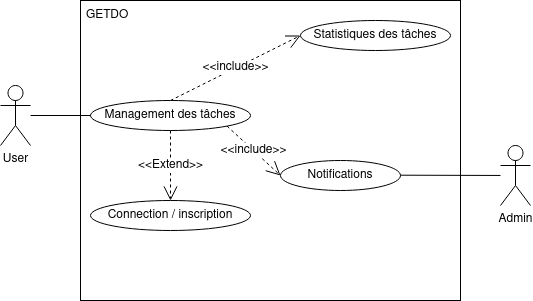
\includegraphics[width=1\textwidth]{./images/Diagramme_useCase.drawio.png}
    \caption{Diagramme de cas d'utilisation de GETDO}
    \label{fig:GETDO_UseCaseDiagramm}
\end{figure}
%---

% usecase diagramm description
\textbf{Système:} Système de gestion de tâches\\
\textbf{Acteurs:}
\begin{itemize}
    \item Utilisateur: Utilise le système pour créer, gérer et suivre ses tâches.
    \item Administrateur: Gère les utilisateurs, les paramètres du système et les rapports.
\end{itemize}
\textbf{Cas d'utilisation:}
\begin{itemize}
    \item Connexion/Inscription: L'utilisateur se connecte ou crée un compte.
    \item Gestion des tâches:
        L'utilisateur crée, modifie, supprime et organise ses tâches.
    \item Statistiques des tâches: L'utilisateur génère des rapports (tâches terminées, temps passé, tâches en retard).
    \item Notifications: L'utilisateur consulte les notifications envoyer par l'administrateur
\end{itemize}
\textbf{Relations:}
\begin{itemize}
    \item Utilisateur: Peut utiliser tous les cas d'utilisation.
    \item Administrateur: Peut envoyer des notifications a l'utilisateur.
    \item Gestion des tâches: Inclut les notifications.
    \item Statistiques des tâches: Étend la gestion des tâches.
\end{itemize}

\subsubsection{Senario de cas d'utilisation}

\textbf{Scénario utilisateur:} Création d'une tâche\\
\textbf{Acteur:} Utilisateur\\
\textbf{Cas d'utilisation:} Gestion des tâches\\
\textbf{Objectif:} Créer une nouvelle tâche dans le système.\\

\textbf{Étapes:}
\begin{itemize}
    \item L'utilisateur se connecte au système en utilisant son nom d'utilisateur et son mot de passe.
    \item L'utilisateur sélectionne l'option "Créer une tâche" dans le menu principal.
    \item L'utilisateur entre le titre de la tâche, une description détaillée, la date d'échéance et la priorité de la tâche.
    \item L'utilisateur clique sur le bouton "Enregistrer" pour créer la tâche.
    \item Le système enregistre la tâche et affiche un message de confirmation.
    \item L'utilisateur peut ensuite visualiser la tâche dans sa liste de tâches ou dans son calendrier.
\end{itemize}
\textbf{Variations:}
    L'utilisateur peut définir une date de rappel pour la tâche.
\textbf{Résultat:}
    Une nouvelle tâche est créée dans le système et est visible pour l'utilisateur qui l'a créée et pour les utilisatePlaurs auxquels elle a été attribuée.\\
%---

% Use case plot
\textbf{Scénario utilisateur:} Modification d'une tâche\\
\textbf{Acteur:} Utilisateur\\
\textbf{Cas d'utilisation:} Gestion des tâches\\
\textbf{Objectif:} Modifier une tâche existante dans le système.\\
\textbf{Étapes:}
\begin{itemize}
    \item L'utilisateur se connecte au système en utilisant son nom d'utilisateur et son mot de passe.
    \item L'utilisateur sélectionne la tâche qu'il souhaite modifier dans sa liste de tâches ou dans son calendrier.
    \item L'utilisateur modifie les informations de la tâche, telles que le titre, la description, la date d'échéance, la priorité, les étiquettes, les pièces jointes et les commentaires.
    \item L'utilisateur clique sur le bouton "Enregistrer" pour enregistrer les modifications.
    \item Le système enregistre les modifications et affiche un message de confirmation.
    \item Les modifications de la tâche sont reflétées dans la liste des tâches de l'utilisateur et dans le calendrier.
\end{itemize}
Variations:
\begin{itemize}
    \item L'utilisateur peut modifier l'état de la tâche, par exemple de "En cours" à "Terminée".
    \item L'utilisateur peut modifier la date de rappel de la tâche.
\end{itemize}
\textbf{Résultat:}
    La tâche est modifiée dans le système et les modifications sont reflétées pour tous les utilisateurs qui peuvent voir la tâche.\\

\textbf{Scénario utilisateur:} Suppression d'une tâche\\
\textbf{Acteur:} Utilisateur\\
\textbf{Cas d'utilisation:} Gestion des tâches\\
\textbf{Objectif:} Supprimer une tâche existante du système.\\
\textbf{Étapes:}
\begin{itemize}
    \item L'utilisateur se connecte au système en utilisant son nom d'utilisateur et son mot de passe.
    \item L'utilisateur sélectionne la tâche qu'il souhaite supprimer dans sa liste de tâches ou dans son calendrier.
    \item L'utilisateur clique sur le bouton "Supprimer" pour supprimer la tâche.
    \item Le système affiche une confirmation demandant à l'utilisateur de confirmer la suppression.
    \item L'utilisateur clique sur le bouton "Confirmer" pour supprimer définitivement la tâche.
    \item Le système supprime la tâche et affiche un message de confirmation.
\end{itemize}
Résultat:
    La tâche est supprimée du système et n'est plus visible pour les utilisateurs.
%---

% Application architecture
\subsection{Architecture de l'application}
L'architecture d'une application est cruciale pour assurer sa performance, sa maintenabilité et son évolutivité. Dans le cadre de notre projet, nous avons choisi d'utiliser \textbf{Vue.js} comme framework frontend et \textbf{Firebase} comme solution backend. Cette combinaison, offre une approche modulaire et efficace permettant de répondre rapidement aux besoins des utilisateurs tout en garantissant une intégration fluide des différentes fonctionnalités. Dans cette, section nous allons détailler les composants clés de l'architecture de l'application ainsi que les interactions entre le frontend et le backend, afin de mieux comprendre les choix techniques effectués et leur impact sur le développement global du.

\subsubsection{frontend}
Le frontend d'une application constitue l'interface, utilisateur celle par laquelle les utilisateurs interagissent directement avec les fonctionnalités. proposées Dans notre, projet nous avons opté pour.Vue, js un framework JavaScript reconnu pour sa flexibilité et sa capacité à créer des interfaces dynamiques et. réactives Cette section explore les principaux composants du, frontend y compris la structure des
composants.

\textbf{Liste des vues:}
\begin{itemize}
    \item\textbf{vue d accueil:} LandingVue
    \item\textbf{ Vue'd inscription:} InscriptionVue
    \item\textbf{ Vue de connection:} ConnectionVue
    \item\textbf{ vue des tâches:} HomeVue
    \item\textbf{ vue du vision bord:} VisionBordVue
    \item\textbf{ vue du calendrier:} CalendarVue
    \item\textbf{ vue du dashbord:} DashbordVue
\end{itemize}
    
\textbf{Liste des composants:}
   \begin{itemize}
    \item HeaderComponent
    \item TaskComponent
    \item VisionComponent\\ \\
   \end{itemize}
    
\textbf{Structure La structure du frontend de l'application:} 
  % application Use case diagramm
  \begin{figure}[h!]
      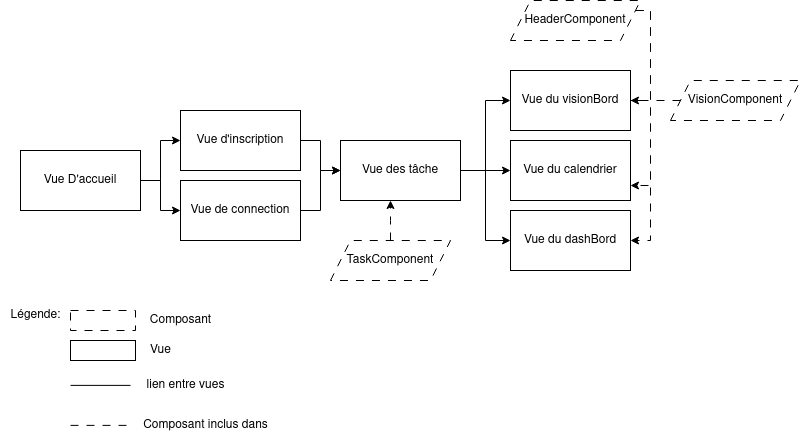
\includegraphics[width=1\textwidth]{./images/getdo_structure_vue.drawio.png}
      \caption{Structure des vues de'l}
      \label{fig:GETDO_UseCaseDiagramm}
  \end{figure}
% ---

\subsubsection{Backend}
Le backend d'une application est essentiel pour gérer les données, l'authentification et la logique métier qui soutiennent le fonctionnement de l'interface utilisateur. Dans notre projet, nous avons choisi Firebase comme solution backend, qui offre une gamme complète de services intégrés pour simplifier le développement. Nous nous pancheront sur les principaux composants du backend, y compris l'authentification des utilisateurs et les bases de données en expliquant comment ils interagissent pour garantir la sécurité, la scalabilité et la performance de l'application. Grâce à Firebase, nous avons pu tirer parti d'une architecture serverless, permettant ainsi une intégration efficace et rapide des fonctionnalités nécessaires à notre projet.

\subsubsection{Présentation Générale de Firebase}

\begin{figure}[h!]
  \centering
  
\includegraphics[width=0.5\textwidth]{./images/firebase.png}
  \caption{firebase}
  \label{fig:Firebase}
\end{figure}

Firebase est une plateforme complète qui fournit tout ce dont vous avez besoin pour créer, développer et gérer des applications mobiles et web performantes.
Avec ses outils puissants et faciles à utiliser, Firebase permet aux développeurs de gagner du temps et de se concentrer sur la création de fonctionnalités innovantes plutôt que sur la gestion de l'infrastructure sous-jacente. Firebase, dispose des fonctionalité suivante:
\begin{itemize}
  \item Authentification : Gérer les connexions des utilisateurs et fournir un accès sécurisé aux données
  \item Bases de données : Stocker et gérer des données structurées et non structurées
  \item Stockage : Stocker et gérer des fichiers tels que des images, des vidéos et des documents
  \item Fonctions cloud : Exécuter du code sans serveur en réponse à des événements
  \item Notifications push : Envoyer des notifications aux utilisateurs sur leurs appareils
  \item Analyse : Suivre les performances de l'application et le comportement des utilisateurs
\end{itemize}

\subsubsection{Interaction frontend-backend}
L'interaction entre le frontend et le backend est cruciale pour les applications web modernes. Dans notre projet, nous utilisons Vue.js pour le frontend et Firebase pour le backend. Vue.js permet de créer des interfaces utilisateur interactives et performantes, tandis que Firebase offre une solution complète incluant l'authentification, la gestion de bases de données en temps réel, et le stockage. Les details d'intéraction se feront comme illustré si desous:
\begin{figure}[h!]
    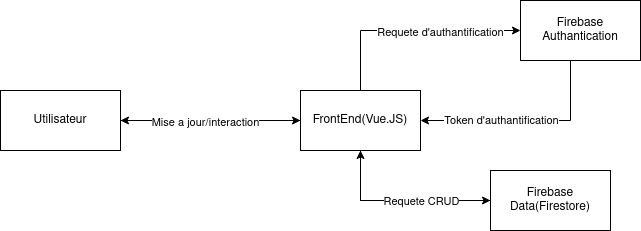
\includegraphics[width=1\textwidth]{./images/backfront-interaction.png}
    \caption{Interaction frontend-backend}
    \label{fig:jira_project_task}
    \end{figure}
\begin{itemize}
  \item \textbf{Utilisateur à Vue.js} : L'utilisateur interagit avec l'interface Vue.js.
  \item \textbf{Vue.js à Firebase Authentication} : Vue.js envoie des requêtes d'authentification pour vérifier l'utilisateur.
  \item \textbf{Firebase Authentication à Vue.js} : Firebase Authentication renvoie un token d'authentification.
  \item \textbf{Vue.js à Firebase Database} : Vue.js envoie des requêtes CRUD (Create, Read, Update, Delete) à la base de données Firebase.
  \item \textbf{Firebase Database à Vue.js} : Firebase Database renvoie les réponses des opérations CRUD.
  \item \textbf{Vue.js à Utilisateur} : Vue.js met à jour l'interface utilisateur avec les données reçues.
\end{itemize}


\subsection{Identité visuelle du project}
L'identité visuelle est l'élément crucial qui donne vie à la personnalité et aux valeurs d'un projet. Elle constitue la première impression que les utilisateurs auront de votre application et joue un rôle essentiel dans la création d'une expérience utilisateur cohérente et engageante.

Cette section du plan de projet s'attache à définir les principes fondamentaux qui guideront la création de l'identité visuelle de l'application. Elle couvrira les aspects suivants :

\begin{itemize}
  \item \textbf{Logo et charte graphique:} Définir les éléments visuels clés qui représentent l'identité de l'application, tels que le logo, la palette de couleurs, la typographie et les images.
  
  \item \textbf {Directives de style:} Établir des règles claires et cohérentes pour l'utilisation de l'identité visuelle dans tous les supports de communication, y compris l'interface utilisateur, les documents marketing et les supports promotionnels.
\end{itemize}
\subsubsection{Logo et charte graphique}
Le logo et la charte graphique sont les piliers fondamentaux de l'identité visuelle d'un projet. Ils constituent la représentation visuelle de la marque et jouent un rôle crucial dans la communication des valeurs, de la mission et de la personnalité du projet auprès du public cible.

% GETDO logo
\begin{figure}[h!]
    
\includegraphics[width=1\textwidth]{./images/GETDO_logo.png}
    \caption{Logo de GETDO}
    \label{fig:jira_project_task}
\end{figure}
%---

\subsubsection{Directive de style}
Dans le cadre de l'implémentation de notre application web, il est essentiel d'adopter une approche cohérente et structurée. Cette section présente les directives de style que nous avons suivies tout au long du projet. Ces règles visent à assurer une expérience utilisateur optimale. En suivant ces directives, nous avons pu créer, répondant aux besoins des utilisateurs tout en respectant les meilleures pratiques de développement web.
\begin{itemize}
  % palette de couleur
  \item\textbf{Palette de couleur principale}:
  \begin{figure}[h!]
    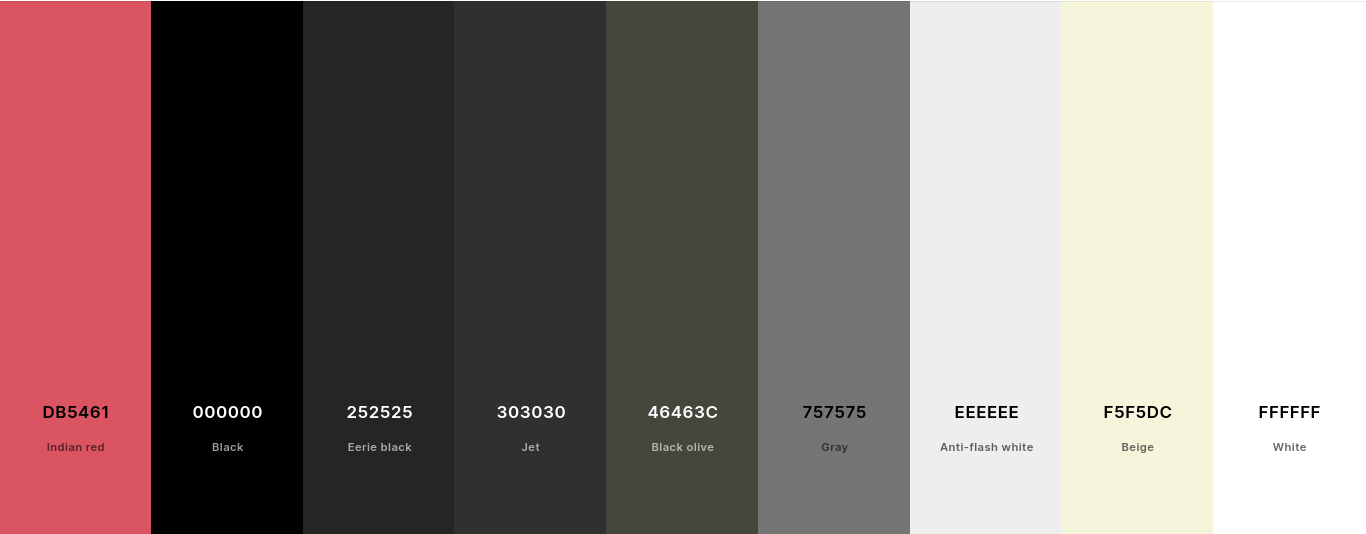
\includegraphics[width=1\textwidth]{./images/getdo-color-palette.png}
    \caption{Palette de couleur principale}
    \label{fig:jira_project_task}
  \end{figure}\\ \\ \\ \\ \\ \\ \\ \\ \\ \\ \\ \\
  %---
 De gauche a droite nous avons:
  \begin{itemize}
    \item\textbf{Indian red(DB5461)}: Uiliser comme couleur principale de l'application
    \item\textbf{Black(000000)}:Couleur des zone de texte en mode sombre et du texte en mode claire.
    \item\textbf{Eerie black(252525)}:Couleur des espaces dans les boites de dialogue.
    \item\textbf{gauche a droite nous avons:Jet(303030)}:Couleur des boites de dialogue (en mode sombre)
    \item\textbf{Black olive(46463C)}:Couleur d'arrière plan (en mode sombre)
    \item\textbf{Grey(757575)}:Couleur des liens
    \item\textbf{Anti-flash white(EEEEEE)}:Couleur des boites de dialogue (en mode clair)
    \item\textbf{Beige(F5F5DC)}:Couleur d'arrière plan (en mode claire)
    \item\textbf{White(FFFFFF)}:Couleur des zone de texte en mode claire et du texte en mode sombre.
  \end{itemize}
  
  \item\textbf{palette de couleur secondaire}: Celle ci sera utiliser pour les indicateurs de niveaux d'importance des tâches
  % palette de couleur secondaire
  \begin{figure}[h!]
    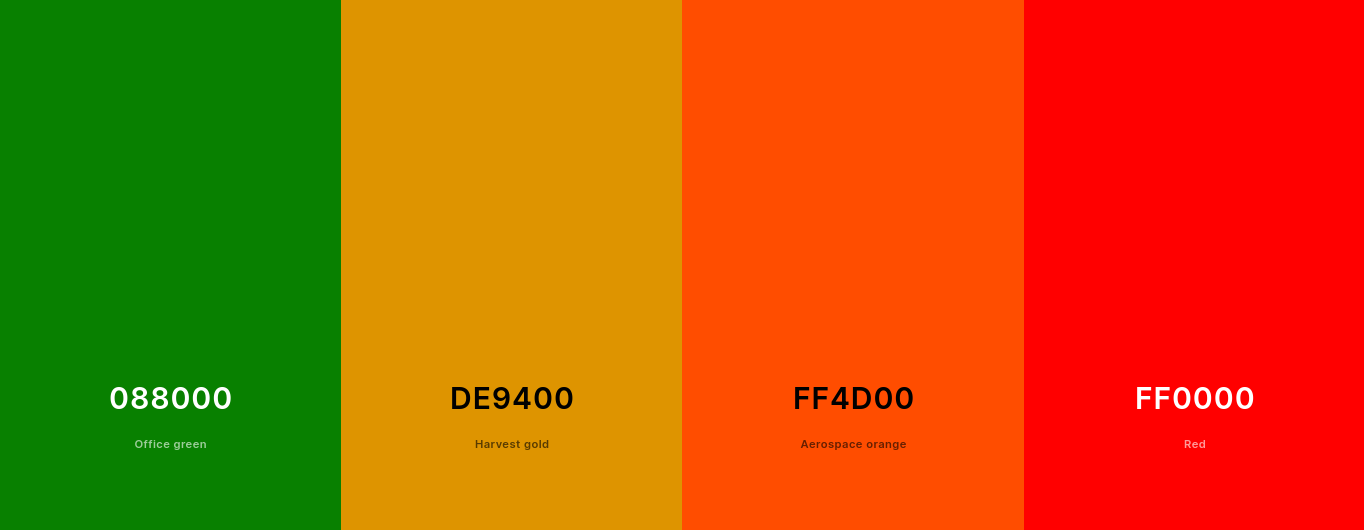
\includegraphics[width=1\textwidth]{./images/getdo-color-palette-indicator.png}
    \caption{Palette de couleur secondaire}
    \label{fig:jira_project_task}
  \end{figure}\\ \\ \\
  %---
  \end{itemize}
  De gauche a droite nous avons:
  \begin{itemize}
    \item\textbf{Office green(088000)}: Pour les tâches de moindre importance.
    \item\textbf{Harvest gold(DE9400)}: Pour les tâches d'importance faible.
    \item\textbf{Aerospace orange(FF4D00)}: Pour les tâches importante.
    \item\textbf{Red(FF0000)}: Pour les tâches urgente.
  \end{itemize}

  \chapter{Analyse des resultats}
  Dans ce chapitre, nous nous pencherons sur l'analyse des résultats obtenus suite à l'implémentation de notre application de gestion de tâches. Cette phase d'analyse est cruciale pour évaluer l'efficacité, la performance et la convivialité de l'application, ainsi que pour identifier les éventuels axes d'amélioration.
  Nous commencerons par examiner les objectifs initiaux du projet et comparerons ces objectifs avec les résultats atteints. Cela nous permettra de déterminer dans quelle mesure les attentes ont été satisfaites et d'évaluer l'impact réel de l'application sur la gestion des tâches.
  Enfin, nous explorerons les avantages et les limitations de l'utilisation de Vue.js et Firebase dans le contexte de ce projet. Cette section fournira un retour d'expérience précieux sur le choix de ces technologies pour le développement de l'application.
  
  \section{Évaluation des Objectifs Initiaux}
    \subsection{Objectifs du Projet}
    L'objectif principal de notre projet était de développer une application de gestion de tâches, nommée GETDO, qui offre une expérience utilisateur intuitive et efficace pour la gestion quotidienne des tâches. Pour atteindre cet objectif, nous avons défini plusieurs fonctionnalités clés que l'application devait intégrer.
    
    \begin{itemize}
    
    \item \textbf{Création de Tâche}
    L'une des fonctionnalités fondamentales de GETDO est la création de tâches. L'application devait permettre aux utilisateurs de créer des tâches rapidement et facilement, en fournissant des options pour définir des titres, des descriptions, des dates d'échéance, des priorités et des catégories. Cette fonctionnalité vise à aider les utilisateurs à organiser et prioriser leurs tâches de manière claire et structurée.

    \item \textbf{Vision Board}
    Le Vision Board est une fonctionnalité innovante de GETDO qui permet aux utilisateurs de visualiser leurs tâches sous forme de tableaux interactifs. Cette vue visuelle aide les utilisateurs à obtenir une perspective globale de leurs tâches, à organiser leurs projets de manière visuelle et à suivre l'avancement de leurs objectifs à long terme. Le Vision Board devait offrir une interface glisser-déposer intuitive pour faciliter la gestion des tâches.

    \item \textbf{Tableaux de Bord et Visualisations de Données}
    Pour fournir une vue d'ensemble complète et analytique de la gestion des tâches, GETDO devait intégrer des tableaux de bord et des visualisations de données. Cette fonctionnalité permet aux utilisateurs de visualiser leurs performances, de suivre le progrès de leurs tâches et de générer des rapports. Les tableaux de bord devaient inclure des graphiques et des statistiques sur les tâches accomplies, en cours et en retard, offrant ainsi une vision claire de la productivité des utilisateurs.

    \item \textbf{Prise en Charge de Styles de Gestion des Tâches}
    GETDO devait offrir une flexibilité dans la gestion des tâches en prenant en charge différents styles de gestion. Les utilisateurs pouvaient choisir entre plusieurs méthodes de gestion des tâches, telles que le Kanban, la méthode GTD (Getting Things Done) ou des listes de tâches traditionnelles. Cette flexibilité permet aux utilisateurs d'adopter le style de gestion qui correspond le mieux à leurs besoins et préférences.
    
    \end{itemize}

  
Ces fonctionnalités clés définissaient les objectifs initiaux de notre projet, visant à créer une application de gestion de tâches complète, flexible et adaptée à divers styles de gestion. En atteignant ces objectifs, nous souhaitions offrir une solution qui améliore la productivité et l'organisation des utilisateurs dans leur vie quotidienne et professionnelle.
    \subsection{Résultats Atteints}
    Cette sous-section présente une évaluation des résultats obtenus par rapport aux objectifs initiaux du projet. Nous analyserons les fonctionnalités implémentées et comparerons les résultats atteints avec les attentes définies. Cela nous permettra de mesurer le succès de notre application de gestion de tâches GETDO et de mettre en lumière les points forts ainsi que les aspects nécessitant des améliorations.\\ \\
    
    \begin{itemize}
       
      \item[•]\begin{figure}[h!]
          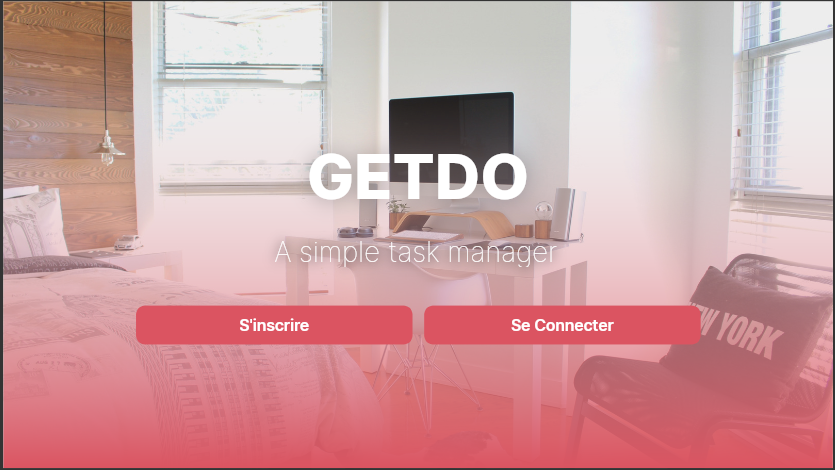
\includegraphics[width=1\textwidth]{./images/getdo_screenshot/getdo_land.png}
          \caption{Page d'accueil}
          \label{fig:jira_project_task}
        \end{figure}
        
      \item[•]\begin{figure}[h!]
          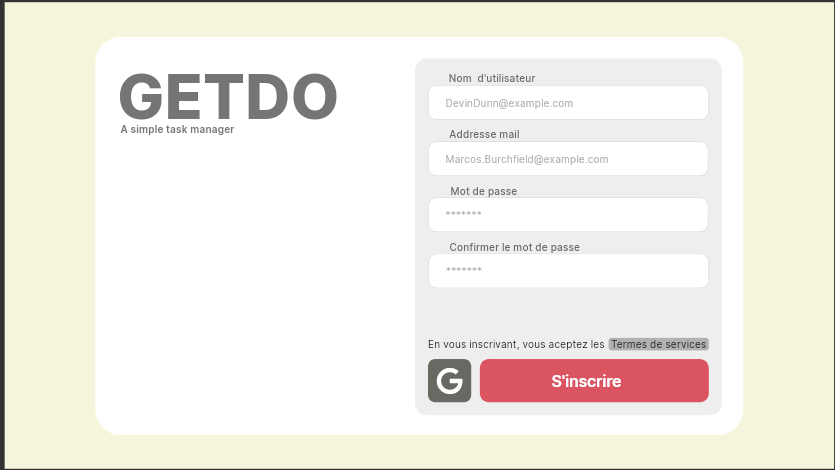
\includegraphics[width=1\textwidth]{./images/getdo_screenshot/getdo_inscription.png}
          \caption{Page d'inscription}
          \label{fig:jira_project_task}
        \end{figure}
        
      \item[•]\begin{figure}[h!]
          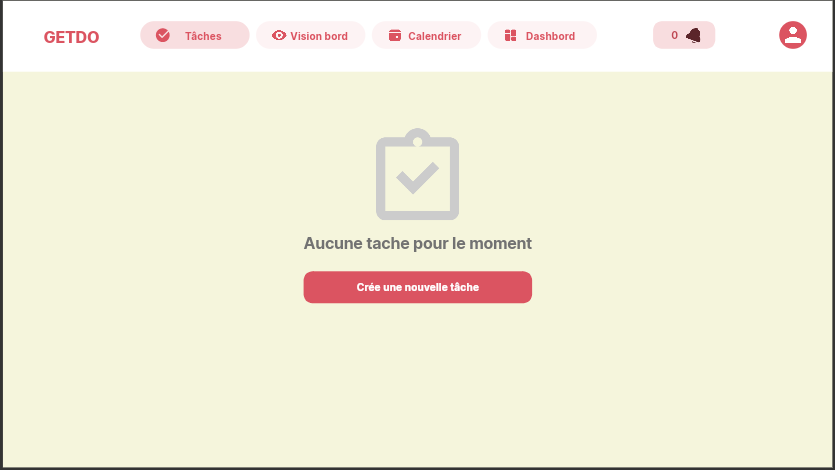
\includegraphics[width=1\textwidth]{./images/getdo_screenshot/getdo_task_empty.png}
          \caption{Page de visualisation de tâche(vide)}
          \label{fig:jira_project_task}
        \end{figure}
        
      \item[•]\begin{figure}[h!]
          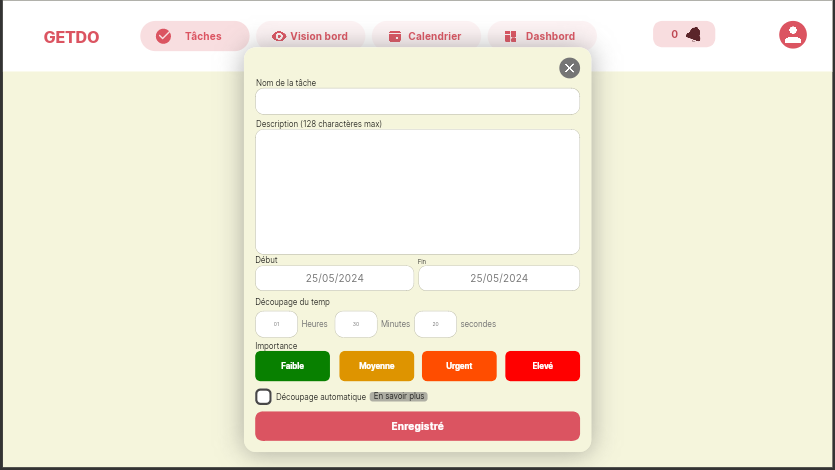
\includegraphics[width=1\textwidth]{./images/getdo_screenshot/getdo_task_form.png}
          \caption{Page de visualisation de tâche(formulaire de creation)}
          \label{fig:jira_project_task}
        \end{figure}
        
      \item[•]\begin{figure}[h!]
          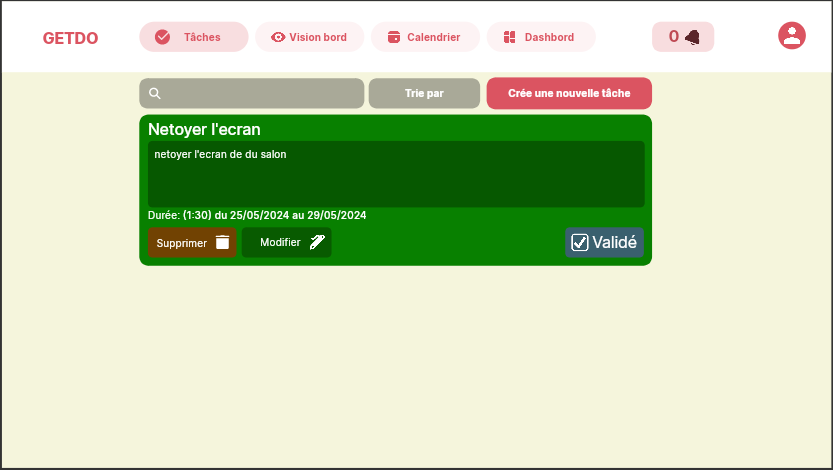
\includegraphics[width=1\textwidth]{./images/getdo_screenshot/getdo_task.png}
          \caption{Page de visualisation de tâche apres creation d'une tâche}
          \label{fig:jira_project_task}
        \end{figure}
        
      \item[•]\begin{figure}[h!]
          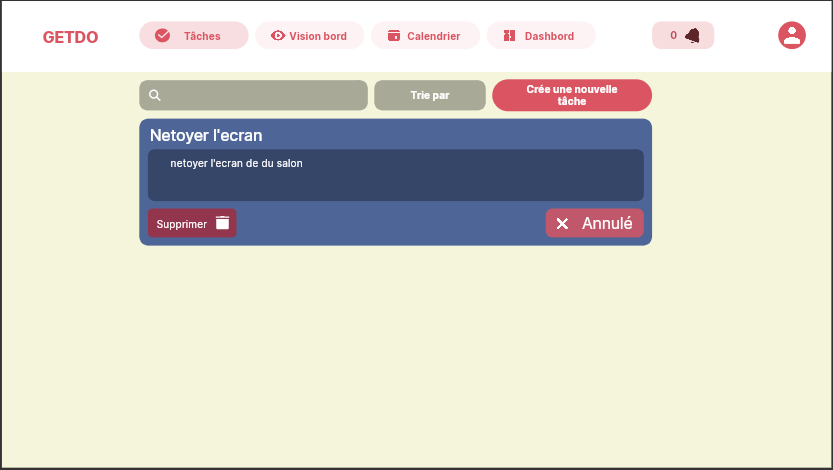
\includegraphics[width=1\textwidth]{./images/getdo_screenshot/getdo_task_finish.png}
          \caption{Tâche apres qu'elle soit terminer}
          \label{fig:jira_project_task}
        \end{figure}
        
      \item[•]\begin{figure}[h!]
          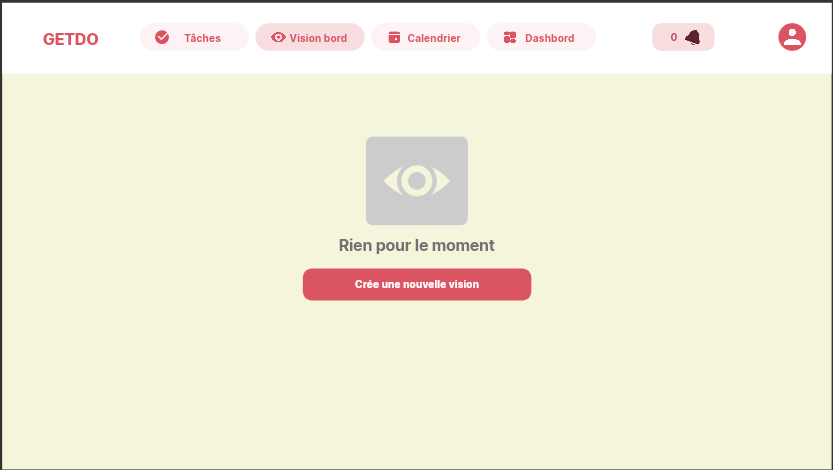
\includegraphics[width=1\textwidth]{./images/getdo_screenshot/getdo_vision_empty.png}
          \caption{Vision bord(vide)}
          \label{fig:jira_project_task}
        \end{figure}
        
      \item[•]\begin{figure}[h!]
          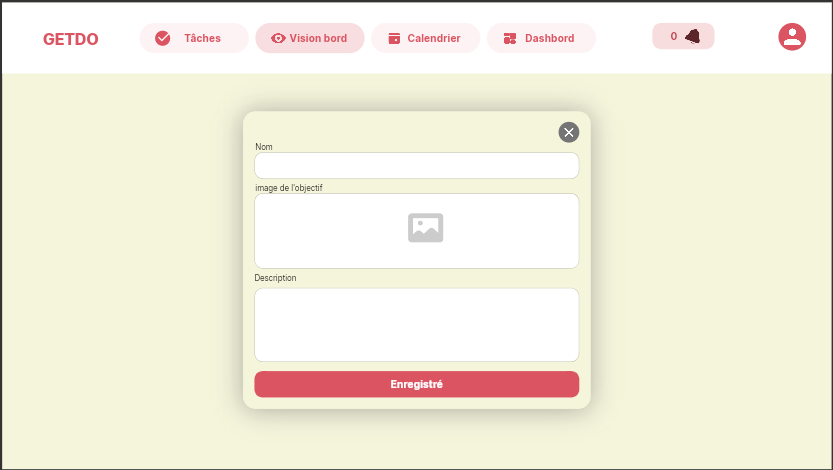
\includegraphics[width=1\textwidth]{./images/getdo_screenshot/getdo_vision_form.png}
          \caption{Vision bord(formulaire de creation)}
          \label{fig:jira_project_task}
        \end{figure}
        
      
      \item[•]\begin{figure}[h!]
          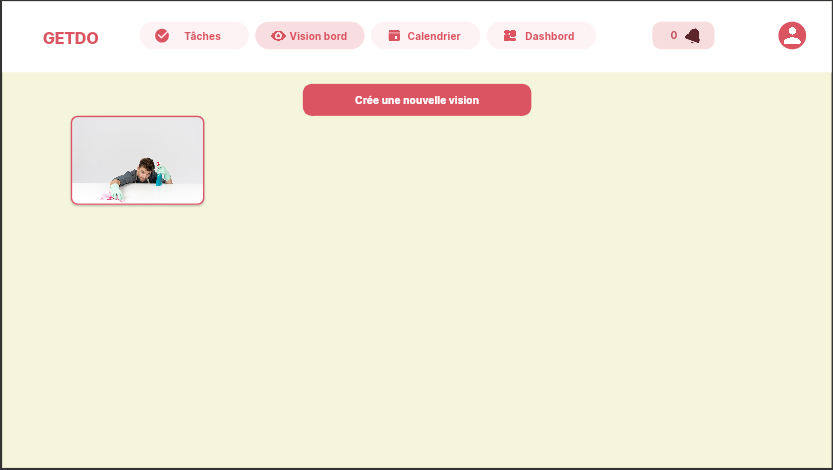
\includegraphics[width=1\textwidth]{./images/getdo_screenshot/getdo_vision.png}
          \caption{Vision bord(photo ajouter)}
          \label{fig:jira_project_task}
        \end{figure}
         
      \item[•]\begin{figure}[h!]
          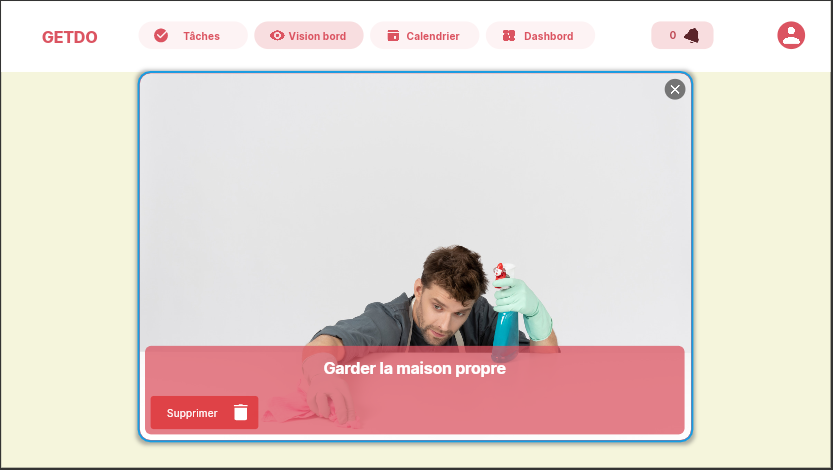
\includegraphics[width=1\textwidth]{./images/getdo_screenshot/getdo_vision_close.png}
          \caption{Vue de plus raproché de la photo et objectif associer}
          \label{fig:jira_project_task}
        \end{figure}
    \end{itemize}
    
  \section{Avantages et Limitations des Technologies Utilisées}
  Dans cette sous-section, nous analyserons les avantages et les limitations des technologies choisies pour le développement de notre application de gestion de tâches, GETDO. L'utilisation de Vue.js pour le frontend et de Firebase pour le backend a offert de nombreux bénéfices, mais aussi posé certains défis. Nous évaluerons comment ces technologies ont contribué à la réalisation de nos objectifs et examinerons les contraintes rencontrées lors de leur mise en œuvre
    \subsection{Avantages de Vue.js}
    Vue.js a été choisi pour le développement du frontend de notre application GETDO en raison de ses nombreux avantages. Voici les principaux bénéfices observés lors de son utilisation :
    \begin{itemize}
      \item\textbf{Facilité d'Apprentissage et d'Utilisation:}Vue.js est réputé pour sa courbe d'apprentissage douce, ce qui a permis à notre équipe de développement de se familiariser rapidement avec le framework. Sa documentation claire et exhaustive a également facilité l'intégration des nouvelles fonctionnalités et la résolution des problèmes rencontrés.
      
      \item\textbf{Performances et Optimisation:}Vue.js est optimisé pour offrir de bonnes performances grâce à son Virtual DOM et à son mécanisme de réactivité. Cela a permis à l'application GETDO de fonctionner de manière fluide, même avec un grand nombre de tâches à gérer, garantissant une expérience utilisateur agréable et sans ralentissement.
      
      \item\textbf{Support Actif et Communauté Vibrante:}
      Vue.js bénéficie d'une communauté active et d'un support continu de la part de ses développeurs. Cette communauté dynamique a fourni de nombreuses ressources, plugins et solutions aux défis rencontrés, accélérant ainsi le développement et la résolution des problèmes.
      
      \item\textbf{Architecture Modulaire et Réactive:}
      Vue.js offre une architecture réactive qui permet de créer des interfaces utilisateur dynamiques et interactives. Sa modularité a facilité la séparation des préoccupations, permettant de structurer l'application en composants réutilisables et maintenables. Cette approche a simplifié le développement et la maintenance de l'application.
      
      \item\textbf{Intégration Facile avec d'Autres Bibliothèques:}
      L'écosystème de Vue.js est conçu pour s'intégrer facilement avec d'autres bibliothèques et outils, tels que Vuex pour la gestion de l'état et Vue Router pour la navigation. Cette flexibilité a permis une adaptation facile aux besoins spécifiques du projet et une extension des fonctionnalités de l'application sans complexité excessive.
    \end{itemize}
    
    \subsection{Avantages de Firebase}
    Firebase, choisi comme backend pour le développement de l'application GETDO, offre une gamme complète de services intégrés qui ont grandement facilité la mise en œuvre du projet. Voici les principaux avantages de l'utilisation de Firebase :
    \begin{itemize}
      \item\textbf{Solution Tout-en-Un:}
      Firebase fournit une suite complète de services backend, incluant la base de données en temps réel (Firestore), l'authentification des utilisateurs, le stockage de fichiers, les fonctions cloud, et bien plus. Cette solution tout-en-un a permis de centraliser les besoins backend en un seul service, simplifiant ainsi le développement et la gestion de l'application.
      
      \item\textbf{Authentification Facile et Sécurisée:}
      Firebase Authentication offre des options simples et sécurisées pour la gestion des utilisateurs, incluant l'authentification par email/mot de passe, l'authentification via des fournisseurs tiers (Google, Facebook, etc.), et la gestion des sessions utilisateur. Cela a permis d'implémenter rapidement des fonctionnalités d'authentification robustes et sécurisées.

      \item\textbf{Fonctionnalités Serverless:}
      Avec Firebase Cloud Functions, il est possible de déployer des fonctions serverless qui réagissent aux événements de la base de données, aux requêtes HTTP, et plus encore. Cette capacité a permis d'implémenter des logiques métiers complexes de manière flexible et évolutive sans avoir à gérer des serveurs dédiés.
      
      \item\textbf{Facilité d'Intégration et Documentation Complète:}
      Firebase dispose d'une documentation exhaustive et d'un support de qualité, facilitant l'intégration rapide des services dans l'application. Cette documentation a été particulièrement utile pour résoudre les problèmes techniques et implémenter les fonctionnalités avancées de manière efficace.
      
    \end{itemize}
    
    \subsection{Limitations de Vue.js et Firebase}

    \subsubsection{Limitations de Vue.js}
    Bien que Vue.js présente de nombreux avantages, certaines limitations ont été rencontrées au  cours du développement de l'application GETDO :
    Courbe d'Apprentissage pour les Concepts Avancés

    \begin{itemize}
      \item\textbf{Complexité Croissante :} Bien que Vue.js soit facile à apprendre pour les débutants, la maîtrise des concepts avancés comme Vuex (gestion d'état), les mixins, et les plugins peut être complexe et nécessiter un temps d'adaptation significatif.

      \item\textbf{Fragmentation des Plugins :} L'écosystème de Vue.js évolue rapidement, ce qui peut entraîner des problèmes de compatibilité entre différentes versions des plugins et des bibliothèques. Cela nécessite une veille technologique constante et peut rendre la maintenance du projet plus difficile.

      \item\textbf{Ralentissement :} Lorsqu'il s'agit de gérer des listes très longues ou des tableaux de données volumineux, Vue.js peut rencontrer des problèmes de performance, malgré l'optimisation du Virtual DOM. Des techniques avancées et des optimisations supplémentaires peuvent être nécessaires pour maintenir une interface fluide.
     \end{itemize}
     
     \subsubsection{Limitations de Firebase}
     Firebase, malgré ses nombreux atouts, présente également certaines limitations qui ont impacté le développement et l'utilisation de l'application GETDO :
     \begin{itemize}
     \item\textbf{Lock-in Technologique :} Firebase est une plateforme propriétaire de Google, ce qui signifie que les développeurs sont en grande partie liés à l'écosystème de Google. Migrer vers une autre solution backend peut être complexe et coûteux en termes de temps et de ressources.

     \item\textbf{Modèle de Tarification :} Bien que Firebase propose une tarification gratuite pour les petits projets, les coûts peuvent rapidement augmenter avec l'échelle et l'usage intensif des services. Les fonctionnalités avancées et les requêtes fréquentes peuvent entraîner des frais importants, surtout pour les startups ou les projets à budget limité.

     \item\textbf{Complexité des Requêtes :} Firestore, bien que puissant, peut rencontrer des limitations lors de la réalisation de requêtes complexes. Les développeurs doivent souvent trouver des solutions de contournement pour des opérations qui seraient triviales avec des bases de données relationnelles traditionnelles.

     \item\textbf{Connexion en Temps Réel :} Firebase dépend d'une connexion Internet stable pour synchroniser les données en temps réel. Dans des environnements où la connectivité est limitée ou instable, cela peut poser des problèmes de synchronisation et d'accès aux données.

     \item\textbf{Règles de Sécurité :} La configuration des règles de sécurité pour Firestore peut être complexe et sujette à des erreurs. Une mauvaise configuration peut entraîner des failles de sécurité potentielles, exposant les données des utilisateurs à des risques.
     \end{itemize}
    
  \section{Perspective d'amelioration}
    \subsubsection{Retour des Utilisateurs}
      \begin{itemize}
      \item\textbf{Feedback Utilisateur Continu :}Mettre en place des mécanismes pour recueillir régulièrement les retours des utilisateurs afin d'identifier les besoins émergents et les points de friction.
      \item\textbf{Mise en Œuvre de Nouvelles Fonctionnalités :} Intégrer de nouvelles fonctionnalités basées sur les retours des utilisateurs, telles que des rappels par notification, des intégrations avec d'autres outils de productivité, ou des options de personnalisation avancées.
      \item\textbf{Intégration du dashbord}: Lors de prochaine mise a jour nous incluront un tableau de visualisation des données
    \end{itemize}
    
    \subsubsection{Amélioration de l'Expérience Utilisateur}
    \begin{itemize}
      \item\textbf{Refonte de l'interface: }Améliorer l'interface utilisateur pour la rendre plus intuitive et accessible, en tenant compte des meilleures pratiques de design UX.
      \item\textbf{Accessibilité :} S'assurer que l'application est accessible à tous les utilisateurs, y compris ceux ayant des besoins spécifiques en matière d'accessibilité.
    \end{itemize}
    
      \subsubsection{Technologies et Outils}
    \begin{itemize}
      \item\textbf{Alternatives Backend :} Évaluer d'autres solutions backend pour compléter ou remplacer certaines fonctionnalités de Firebase, en cas de besoin spécifique ou de contraintes de coût.
      \item\textbf{Mises à Jour et Nouveautés :} Rester à jour avec les dernières versions de Vue.js et Firebase, ainsi que les nouvelles fonctionnalités et améliorations proposées par la communauté et les développeurs de ces technologies.
    \end{itemize}
    
    \subsubsection{Intégration de l'inteligence Artificielle}
    Grace a l'intégration de l'inteligence Artificielle, notre service aura la possibilité de simplifier la creation et gestion de tâche.
    
    En mettant en œuvre ces perspectives d'amélioration, nous visons à continuer à offrir une application de gestion de tâches performante, sécurisée et centrée sur l'utilisateur. Ces efforts contribueront à maintenir la satisfaction des utilisateurs et à assurer la croissance et l'évolution de GETDO dans un environnement technologique en constante évolution.
    
    \chapter*{Conclusion Générale}
    % ---
    En conclusion, ce rapport a détaillé l’ensemble du processus de développement de l’application de gestion de tâches GETDO, allant de la conception initiale à l’évaluation des résultats obtenus. L’objectif principal de ce projet était de créer une solution robuste et intuitive pour aider les utilisateurs à gérer leurs tâches personnelles et professionnelles de manière efficace.

    Nous avons abordé les différentes phases de développement, en mettant en évidence les défis rencontrés et les solutions apportées. Le choix des technologies modernes telles que Vue.js pour le front-end et Firebase pour le back-end a permis de réaliser une application performante, réactive et sécurisée.

    L’analyse des résultats a démontré que les objectifs initiaux du projet ont été atteints, voire dépassés dans certains aspects. L’application GETDO a prouvé son efficacité en termes de gestion de tâches, offrant une interface utilisateur conviviale et des fonctionnalités avancées telles que le Vision Board, les tableaux de bord et les visualisations de données.

    Cependant, nous avons également identifié des limitations et des axes d’amélioration, notamment en ce qui concerne la scalabilité et la gestion des tâches complexes. Ces observations ouvrent des perspectives intéressantes pour des évolutions futures, notamment l’intégration de l’intelligence artificielle pour améliorer encore davantage l’expérience utilisateur et la productivité.

    Enfin, ce projet a été une occasion précieuse d’acquérir des compétences pratiques en développement d’applications web et d’explorer les possibilités offertes par des technologies modernes. Nous espérons que ce travail pourra servir de base pour des projets futurs et contribuer à l’amélioration continue des outils de gestion de tâches.

   \chapter*{Reference bibiographique}
   \begin{itemize}
     \item \url{https://blog.visual-paradigm.com/fr/}
     \item \url{https://firebase.google.com/}
     \item \url{https://coolors.co/}
     \item \url{https://app.diagrams.net/}
     \item \url{https://vuefire.vuejs.org/}
     \item \url{https://www.overleaf.com/}
     \item \url{https://www.latex-fr.net/}
     \item \url{https://www.digitalocean.com/}
   \end{itemize}
    

\end{document}